%% GENERIC STYLE SETTINGS
\usetheme{default}
\usepackage{listings}
\usepackage{multirow}
\usepackage{xcolor}

\usebackgroundtemplate{

\includegraphics[width=\paperwidth,height=\paperheight]{images/hutton_background}
}
%% PRESENTATION CONFIGURATION PARAMETERS %%%%%%%%%%%%%%%%%%%%%%%%%%%%%%%%%%%%%%%
%\titlebackgroundfile{images/hutton_title}
%\framebackgroundfile{images/hutton_background}
\definecolor{hutton_green}{HTML}{78A22F}
\definecolor{hutton_purple}{HTML}{872175}
\definecolor{hutton_blue}{HTML}{569BBE}
\usefonttheme{structurebold}
\setbeamercolor{alerted text}{fg=orange}
\setbeamercolor{background canvas}{bg=white}
\setbeamercolor{block title}{bg=hutton_purple}
\setbeamercolor{frametitle}{fg=hutton_purple}
\setbeamercolor{title}{fg=black}
\setbeamercolor{titlelike}{fg=hutton_green}
\setbeamercolor{author}{fg=hutton_purple}
\setbeamercolor{author in head/foot}{fg=white}
\setbeamercolor{title in head/foot}{fg=white}
\setbeamercolor{section in head/foot}{fg=hutton_purple}
\setbeamercolor{normal text}{fg=black}
\setbeamercolor{frametitle}{fg=hutton_purple}
\setbeamerfont{block title}{size={}}
\setbeamerfont{author}{size=\footnotesize}
\setbeamerfont{date}{size=\footnotesize}
\setbeamercolor{section in toc shaded}{fg=hutton_purple}
\setbeamercolor{section in toc}{fg=hutton_purple}
\setbeamercolor{subsection in toc shaded}{fg=hutton_purple}
\setbeamercolor{subsection in toc}{fg=hutton_purple}
\setbeamertemplate{itemize item}[circle]
\setbeamertemplate{itemize subitem}[circle]
\setbeamertemplate{itemize subsubitem}[circle]
\setbeamertemplate{itemize subsubsubitem}[circle]
\setbeamercolor{itemize item}{fg=hutton_purple}
\setbeamercolor{itemize subitem}{fg=hutton_purple}
\setbeamercolor{itemize subsubitem}{fg=hutton_purple}
\setbeamercolor{itemize subsubsubitem}{fg=hutton_purple}
\setbeamercolor{enumerate item}{fg=hutton_purple}
\setbeamercolor{enumerate subitem}{fg=hutton_purple}
\setbeamercolor{enumerate subsubitem}{fg=hutton_purple}
\setbeamercolor{enumerate subsubsubitem}{fg=hutton_purple}
\setbeamercolor{alerted text}{fg=hutton_green}
\setbeamerfont{alerted text}{series=\bfseries}
% This command makes that acrobat reader doesn't changes the colors of the slide
% when there are figures with transparencies.
\pdfpageattr {/Group << /S /Transparency /I true /CS /DeviceRGB>>}

%Disables discrete bottom navigation bar
%\beamertemplatenavigationsymbolsempty

%Mess about with the slide titles to avoid the corner images,
\setbeamertemplate{frametitle}
{
\vspace{0.05\textheight}
\noindent\quad\begin{minipage}[t][0.12\textheight][t]{0.85\textwidth}
\insertframetitle\par
\end{minipage}
}

%Mess about with title page to avoid the big logo on right
\setbeamertemplate{title page}{
    \begin{picture}(0,0)
            %This ends up on top of the default background image, rather than replacing it:
            \put(-30,-165){%
                
\includegraphics[width=\paperwidth,height=\paperheight]{images/hutton_title}
            }
            \put(0,-75){%
                \begin{minipage}[b][0.4\textheight][t]{0.75\textwidth}
                    \usebeamerfont{title}\usebeamercolor[fg]{title}{\inserttitle\par}
                    \usebeamerfont{subtitle}\usebeamercolor[fg]{subtitle}{\insertsubtitle\par}
                \end{minipage}
            }
            \put(0,-135){%
                \begin{minipage}[b][0.1\textheight][t]{\textwidth}
                    \usebeamerfont{author}\usebeamercolor[fg]{author}{\insertauthor\par}
                \end{minipage}
            }
    \end{picture}
}

%%%%%%%%%%%%%%%%%%%%%%%%%%%%%%%%%%%%%%%%%%%%%%%%%%%%%%%%%%%%%%%%%%%%%%%%%%%%%%%%

% LISTINGS SETTING
% Settings for code listings in lstlistings

\lstset{ %
  backgroundcolor=\color{yellow},   % choose the background color; you must add \usepackage{color} or \usepackage{xcolor}
  basicstyle=\tiny\ttfamily,        % the size of the fonts that are used for the code
  breakatwhitespace=false,         % sets if automatic breaks should only happen at whitespace
  breaklines=true,                 % sets automatic line breaking
  captionpos=b,                    % sets the caption-position to bottom
  commentstyle=\color{red},    % comment style
  deletekeywords={...},            % if you want to delete keywords from the given language
  escapeinside={\%*}{*)},          % if you want to add LaTeX within your code
  extendedchars=true,              % lets you use non-ASCII characters; for 8-bits encodings only, does not work with UTF-8
  frame=single,                    % adds a frame around the code
  keepspaces=true,                 % keeps spaces in text, useful for keeping indentation of code (possibly needs columns=flexible)
  keywordstyle=\color{blue},       % keyword style
%  language=Octave,                 % the language of the code
  morekeywords={*,...},            % if you want to add more keywords to the set
  numbers=left,                    % where to put the line-numbers; possible values are (none, left, right)
  numbersep=5pt,                   % how far the line-numbers are from the code
  numberstyle=\tiny\color{gray}, % the style that is used for the line-numbers
  rulecolor=\color{black},         % if not set, the frame-color may be changed on line-breaks within not-black text (e.g. comments (green here))
  showspaces=false,                % show spaces everywhere adding particular underscores; it overrides 'showstringspaces'
  showstringspaces=false,          % underline spaces within strings only
  showtabs=false,                  % show tabs within strings adding particular underscores
  stepnumber=1,                    % the step between two line-numbers. If it's 1, each line will be numbered
  stringstyle=\color{violet},     % string literal style
  tabsize=4,                       % sets default tabsize to 2 spaces
  title=\lstname                   % show the filename of files included with \lstinputlisting; also try caption instead of title
}


%%%
% TITLE PREAMBLE
\title[Intro to Bioinformatics] % (optional, only for long titles)
{Introduction to Bioinformatics}
\subtitle{Part 0: So You Want To Be a Computational Biologist?}
\author[Pritchard, Cock] % (optional, for multiple authors)
{Leighton~Pritchard and Peter~Cock}
\institute[The James Hutton Institute] % (optional)
{
  Information and Computational Sciences\\
  The James Hutton Institute
}
\date[May, June, August, December 2014] % (optional)
{Bioinformatics Training, 29$^{th}$, 30$^{th}$ May, 5$^{th}$ June, 11$^{th}$ August, $9^{th}$ December 2014}
\subject{Bioinformatics}

%%%
% TOC
% Show table of contents, with current section highlighted,
% at the start of each section

\AtBeginSection[]
{
  \begin{frame}
    \frametitle{Table of Contents}
    \tableofcontents[currentsection,hideallsubsections]
  \end{frame}
}

%%%
% START DOCUMENT
\begin{document}

\frame[plain]{\titlepage}

% Bertrand Russell quote
% Image of Bertrand Russell quote:
% "It is not what the man of science believes that distinguishes him,
%  but how and why he believes it.
%  His beliefs are tentative, not dogmatic; they are based on evidence,
%  not on authority or intuition."
\begin{frame}
  \frametitle{Bertrand Russell}
  \begin{center}
    
\includegraphics[width=\textwidth]{images/bertrand}
  \end{center}
\end{frame}
    
%%%
% SECTION: Introduction
\section{Introduction}
  % So You Want To Be a Computational Biologist
%
% A brief introduction to emphasise that bioinformatics is biology,
% even if a particular skill set, and that acquiring that skill set will
% need practice.

\subsection{So You Want To Be a Computational Biologist?}
\begin{frame}
  \frametitle{What is this ``bioinformatics'' thing, anyway?}
  \begin{itemize}
    \item Bioinformatics: biology using computational and mathematical tools
    \item A discipline within biology
    \begin{itemize}
      \item Loman \& Watson (2013) ``So you want to be a computational biologist?''
        \url{http://dx.doi.org/10.1038/nbt.2740}
      \item Welch \textit{et al.} (2014) ``Bioinformatics Curriculum Guidelines: Toward a Definition of Core Competencies''
      \url{http://dx.doi.org/10.1371/journal.pcbi.1003496}
      % http://bit.ly/1fS4iDJ links to http://biomickwatson.wordpress.com/2014/03/10/the-only-core-competency-youre-ever-going-to-need/}
      \item Watson (2014) ``The only core competency you need'' \url{http://bit.ly/1fS4iDJ} (blog)
    \end{itemize}
  \end{itemize}
\end{frame}

\subsection{So You Want To Be a Computational Biologist?}
\begin{frame}
  \frametitle{What is this ``bioinformatics'' thing, anyway?}
  
\includegraphics[width=.5\textwidth]{images/twitter_bioinformatician}
  
\includegraphics[width=.5\textwidth]{images/twitter_computers_biology}  
\end{frame}

\subsection{So You Want To Be a Computational Biologist?}
\begin{frame}
  \frametitle{Some uncomfortable truths}
  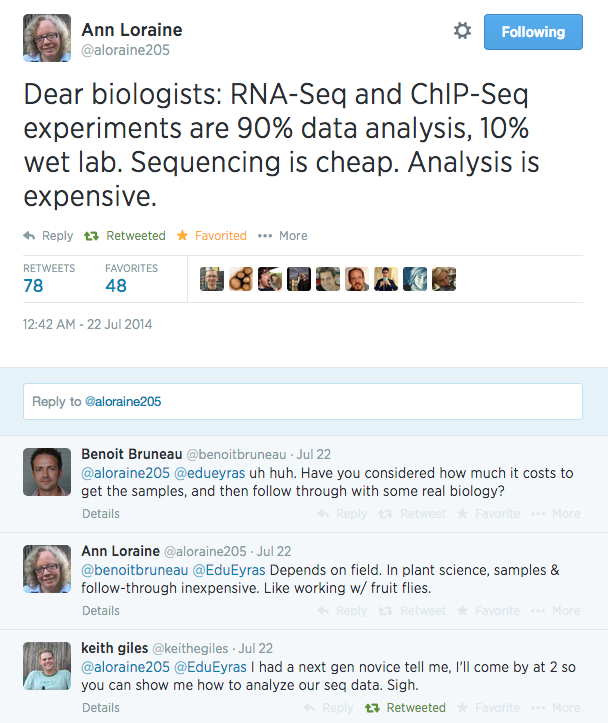
\includegraphics[width=.5\textwidth]{images/twitter_rnaseq}
  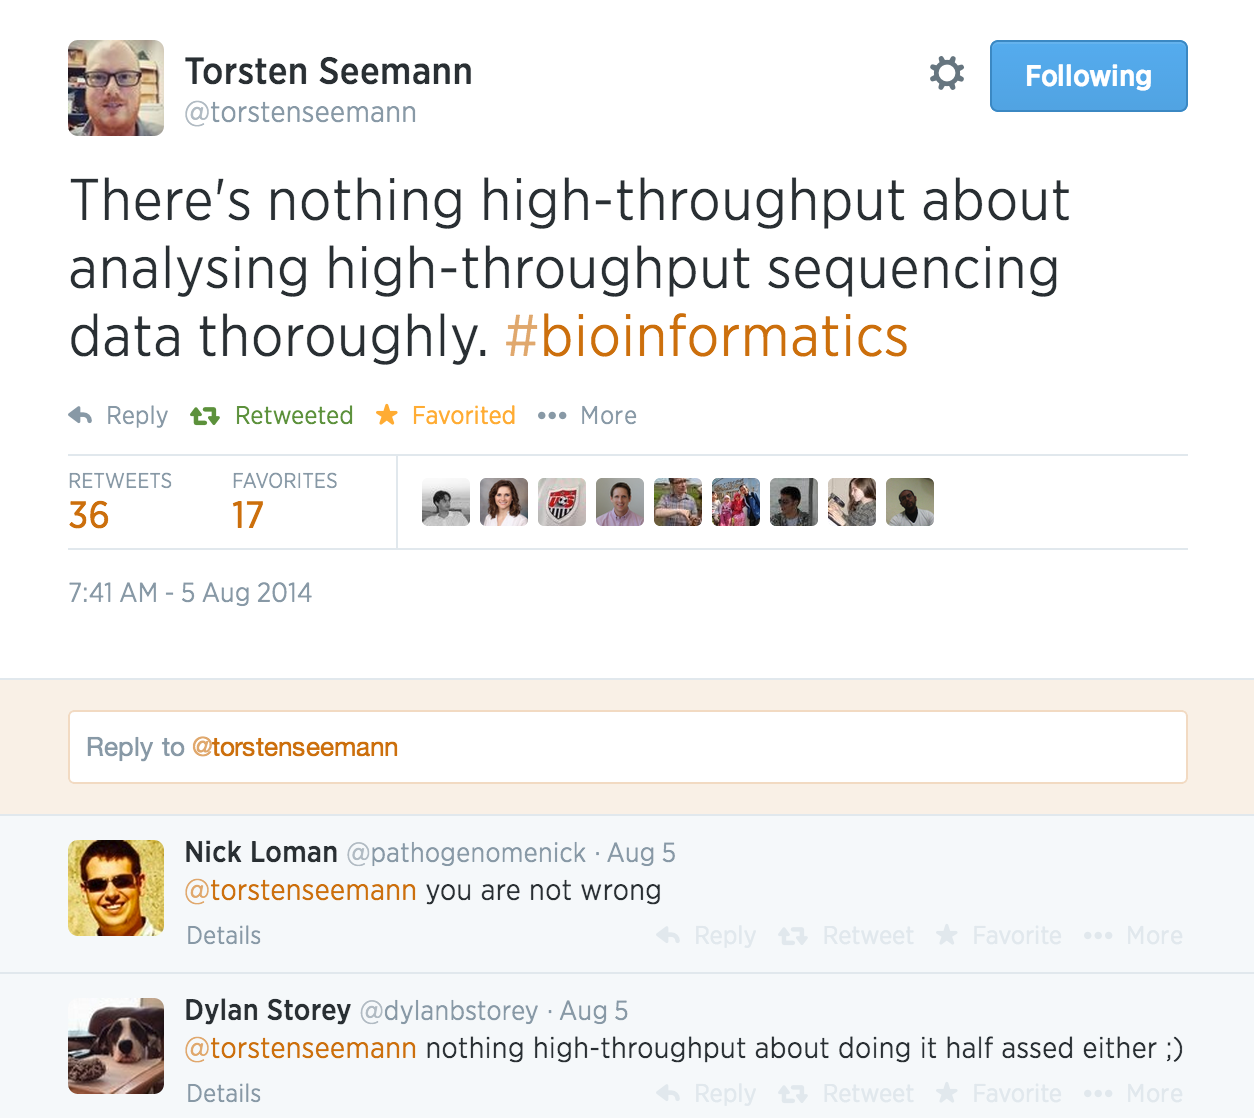
\includegraphics[width=.5\textwidth]{images/twitter_high_throughput}  
\end{frame}

\begin{frame}
  \frametitle{Some uncomfortable truths}
  \begin{itemize}
    \item<1-> This one-day course will not make you a bioinformatician
    \begin{itemize}
      \item<2-> But practice might$\ldots$
    \end{itemize}
    \item<3-> The best way to learn is to do (``I don't know how to do this yet, but I will find out.'')
    % http://bit.ly/Rq0D61 links to http://biomickwatson.wordpress.com/2013/08/06/bioinformatics-is-not-something-you-are-taught-its-a-way-of-life/
    \begin{itemize}
      \item \url{http://bit.ly/Rq0D61} (``Bioinformatics is a way of life'')
    \end{itemize}
    \item<3-> Most bioinformatics is problem-solving
    \item<3-> We will introduce some useful tools and concepts
  \end{itemize}
\end{frame}

\begin{frame}
  \frametitle{What it takes to be a bioinformatician}
  \begin{columns}[t]
    \begin{column}{5cm}
      \begin{itemize}
        \item Patience (problem-solving)
        \item Suspicion (statistics)
        \item Biological knowledge
        \item Social skills (no-one knows everything: ask!)
        \item Lots of practice          
      \end{itemize}
    \end{column}
    \begin{column}{5cm}
      \begin{itemize}
        \item Self-confidence (challenge results and dogma)
        \item Core domain skills: biology, computer science, statistics
        \item Deliver results (qualified, honest)
      \end{itemize}
    \end{column}
  \end{columns}
  \begin{itemize}
  % http://bit.ly/1jDuQsO link goes to http://biomickwatson.wordpress.com/2013/03/18/the-alternative-what-it-takes-to-be-a-bioinformatician/
    \item Watson (2014) ``What it takes to be a bioinformatician'' \url{http://bit.ly/1jDuQsO} (blog)
    %\item \url{http://science.slashdot.org/comments.pl?sid=3161217&cid=41542125}
  \end{itemize}
\end{frame}

\begin{frame}
  \frametitle{More general advice?}
  \begin{itemize}
    \item Ask us (we do this a lot)
    \item BioStars (\url{https://www.biostars.org})
    \item SeqAnswers (\url{http://seqanswers.com/})
    \item \textit{PLoS Comp Biol} collections (\url{http://www.ploscollections.org/static/pcbiCollections})
 \end{itemize}
 
\includegraphics[width=.2\textwidth]{images/gibas_book}
 
\includegraphics[width=.2\textwidth]{images/buffalo_book}
 
\includegraphics[width=.18\textwidth]{images/bassi_book}
 
\includegraphics[width=.2\textwidth]{images/korf_book}
 
\includegraphics[width=.2\textwidth]{images/model_book}
\end{frame}

%%%
% SECTION: Recording your work
\section{Recording Your Work}
  % Recording Bioinformatics Work
%
% A brief set of reasons for why you would want to record your work,
% and record it well.

\subsection{Recording Bioinformatics Work}
\begin{frame}
  \frametitle{Why Do It?}
  \begin{itemize}
    \item Doing bioinformatics is doing science: keep a lab book!
    \item You \emph{will not} remember multiple files, analysis details, etc. in a week/month/six months/a year/three years
    \begin{itemize}
      \item Noble (2009) \url{http://dx.doi.org/10.1371/journal.pcbi.1000424}
      \item Baggerly \& Coombes (2009) \url{http://dx.doi.org/10.1214/09-AOAS291}
    \end{itemize}
  \end{itemize}
  
\includegraphics[width=.6\textwidth]{images/noble_2009_head}
\end{frame}
   
\begin{frame}
  \frametitle{How To Do It? I}
  \begin{itemize}
    \item There is no one correct way, but$\ldots$
    \item Think about data/docs/project structure \textit{before} you start
  \end{itemize}
  \begin{center}
    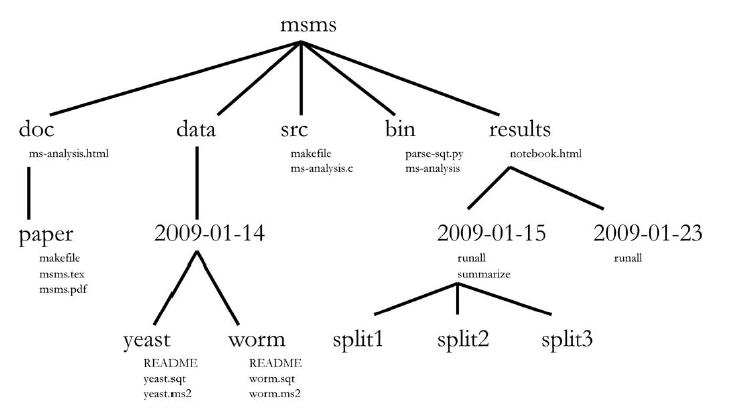
\includegraphics[width=.5\textwidth]{images/project_structure}
    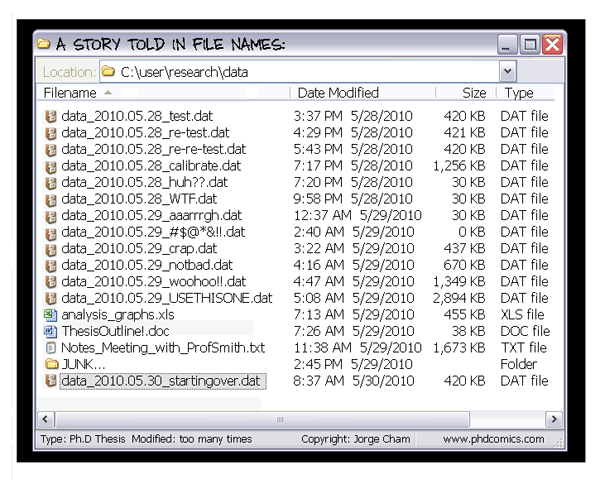
\includegraphics[width=.5\textwidth]{images/phd052810s}
  \end{center}
\end{frame}

\begin{frame}
  \frametitle{How To Do It? II}
  \begin{itemize}
    \item Use plain text where possible
      \item Use version control
      \item Keep backups
      \item Different tools suit different purposes: code \textit{vs.} data \textit{vs.} analysis \textit{vs.} $\ldots$
      \item Find a way that works \emph{for you}.
  \end{itemize}
\end{frame}

\begin{frame}
  \frametitle{How To Do It? III}
  \begin{itemize}
    \item Reproducibility is key!
    \item Scripts and pipelines are better for this than notes of what you did
    \begin{itemize}
      \item Also better for version control, and reuse
    \end{itemize}
    \item Avoid unnecessary duplication
    \begin{itemize}
      \item Someone else may have solved your problem
      \item One (backed up) read-only copy of raw data, keep analyses separate
    \end{itemize}
  \end{itemize}
\end{frame}
   
   
% Useful tools for recording bioinformatics work
  % Useful Tools for Recording Bioinformatics Work
%
% Subsection listing several tools that are useful for recording bioinformatics work

\subsection{Useful Tools for Recording Bioinformatics Work}
\begin{frame}
  \frametitle{Plain Text Files}
  \begin{itemize}
    \item \texttt{README.txt}/\texttt{README.md} in each directory/folder
    \item Plain text is always human-readable
    \begin{itemize}
      \item Markdown (\url{https://daringfireball.net/projects/markdown/basics})
      \item RST (\url{http://docutils.sourceforge.net/docs/ref/rst/restructuredtext.html})
    \end{itemize}
  \end{itemize}
  \begin{center}
    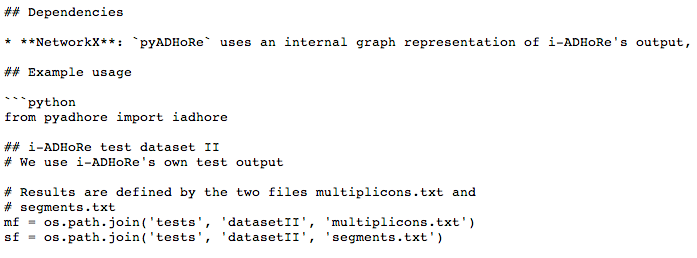
\includegraphics[width=.4\textwidth]{images/markdown_before}
    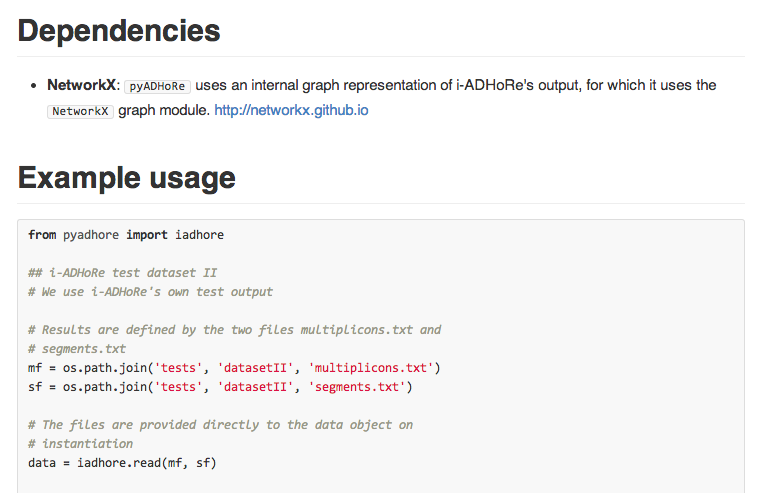
\includegraphics[width=.4\textwidth]{images/markdown_after}
  \end{center}
\end{frame}
   
\begin{frame}
  \frametitle{Galaxy workflows}
  \begin{itemize}
    \item Use through browser, graphical interface
    \item Reproducible, shareable, documentable, reusable analyses
    \item Wraps standard bioinformatics tools
    \item Local instance (\url{http://galaxy.hutton.ac.uk}) uses JHI cluster       
  \end{itemize}
  \begin{center}
    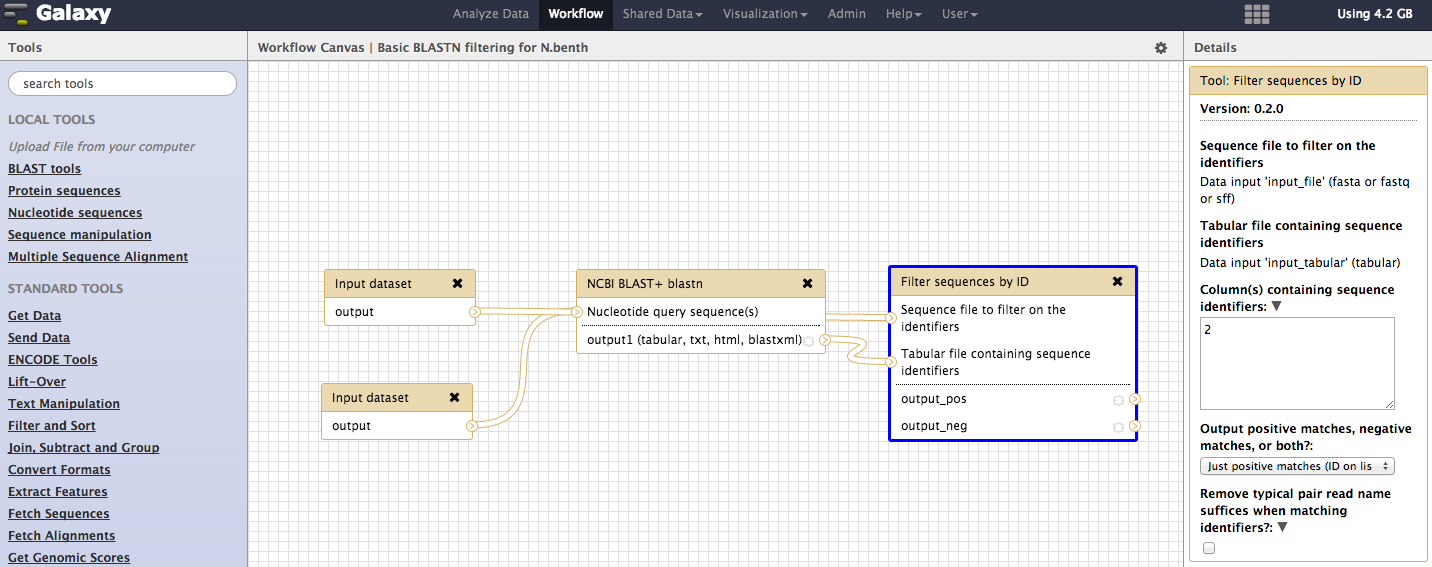
\includegraphics[width=.75\textwidth]{images/galaxy_screenshot}
  \end{center}
\end{frame}      
   
\begin{frame}
  \frametitle{\texttt{script}}
  \begin{itemize}
    \item Writes your terminal activity to a plain text file
    \item Saves effort copy/pasting and typing commands into a lab book, as you go
    \item Easy to use with other tools 
    \item use \texttt{man script} at your terminal to find out more
  \end{itemize}
\end{frame}   
   
\begin{frame}
  \frametitle{MediaWiki}
  \begin{itemize}
    \item Useful for shared projects/data
    \item Automatic version control and attribution
    \item Many local instances at JHI (ask around)
  \end{itemize}
  \begin{center}
    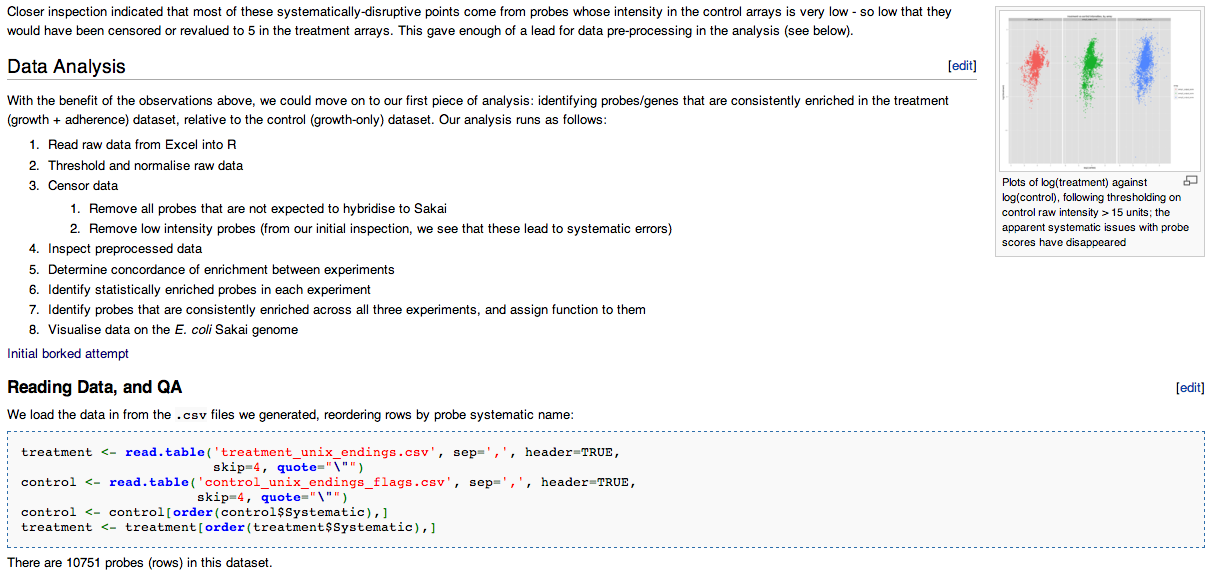
\includegraphics[width=.4\textwidth]{images/mediawiki_after}
    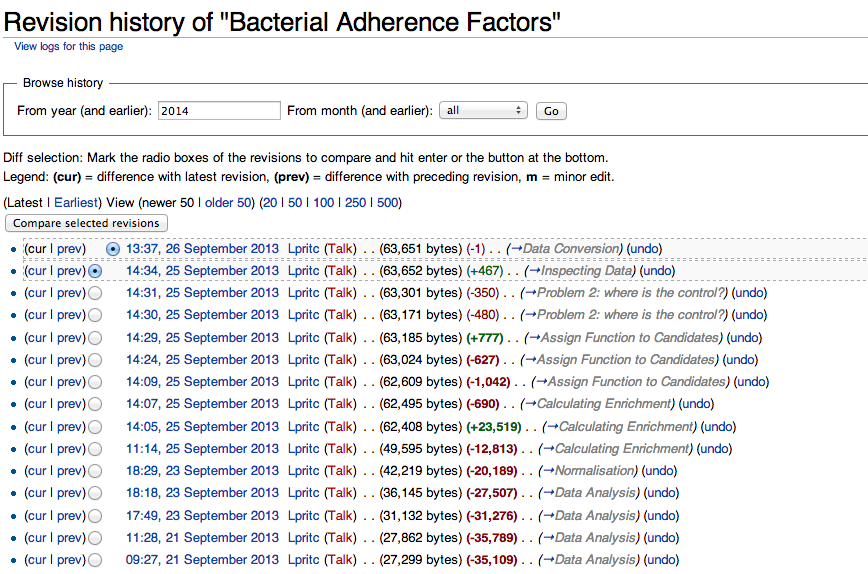
\includegraphics[width=.4\textwidth]{images/mediawiki_version_control}     
  \end{center}
\end{frame}
   
\begin{frame}
  \frametitle{A language notebook}
  \begin{itemize}
    \item e.g. \texttt{iPython Notebook}, \texttt{knitr}, \texttt{Mathematica}, \texttt{MatLab} cells
    \item Integrates live code and analysis with lab-book
  \end{itemize}
  \begin{center}
    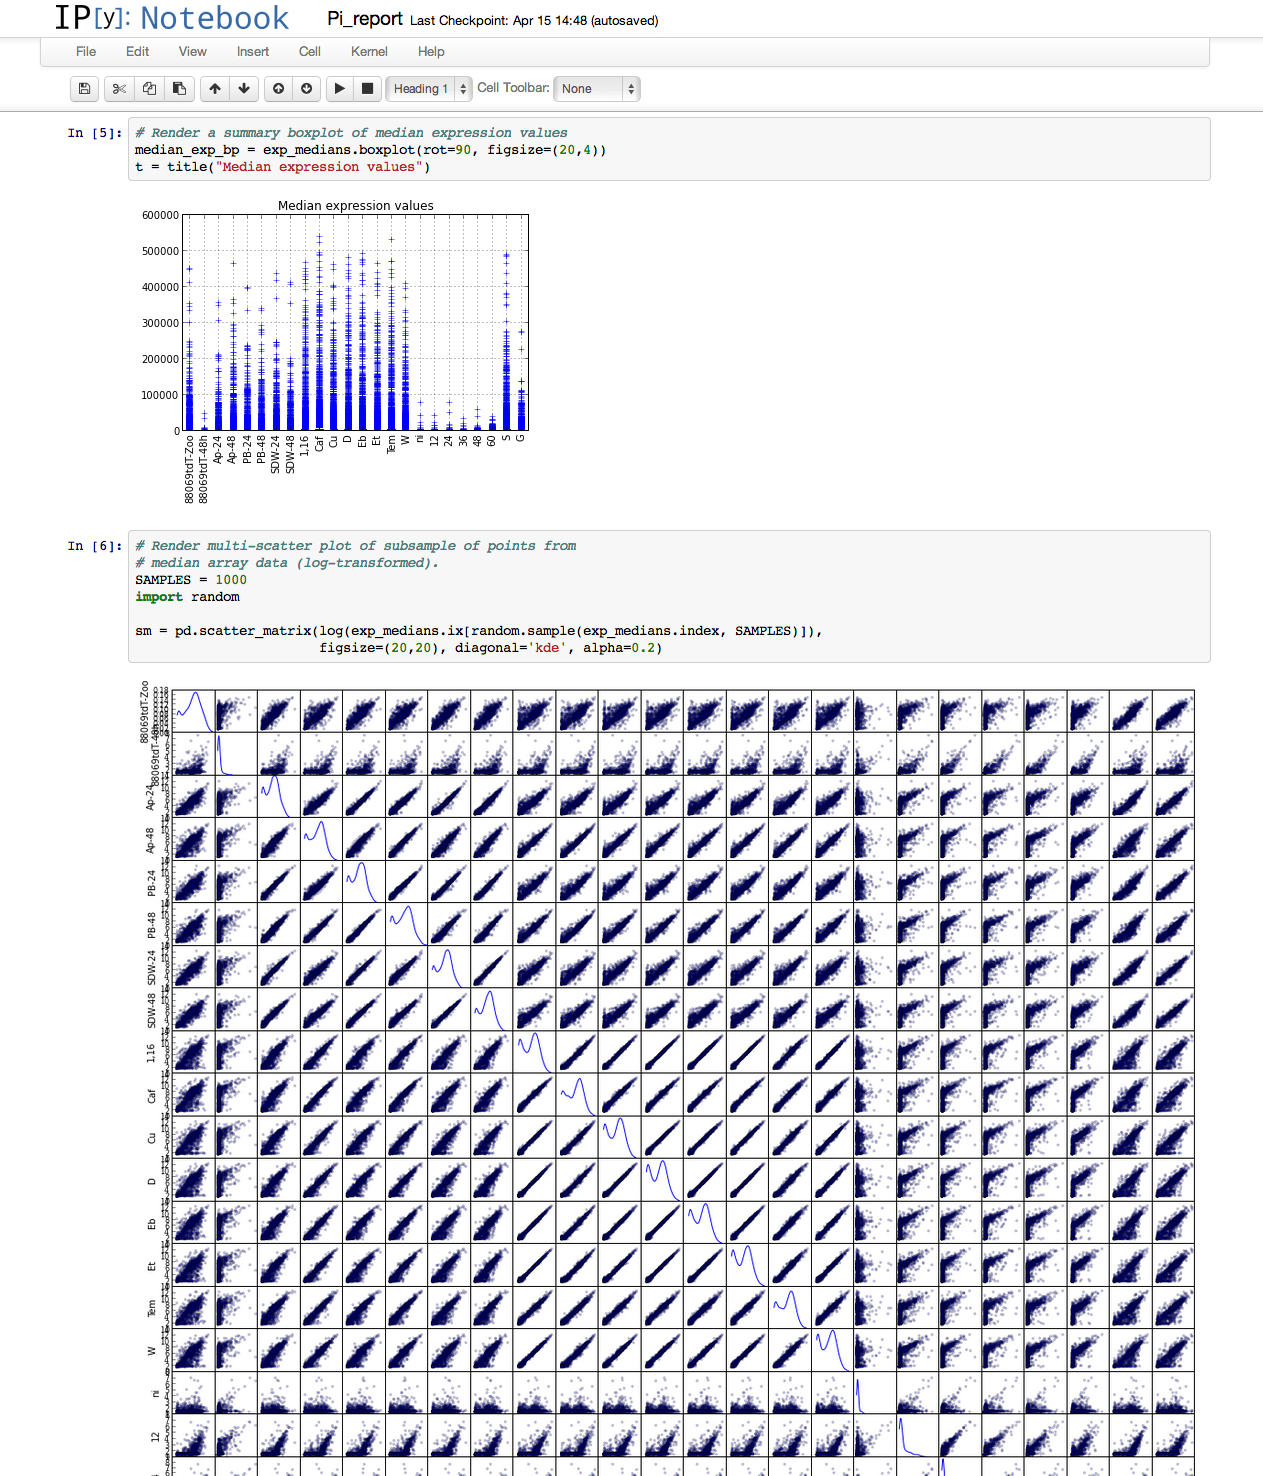
\includegraphics[width=.35\textwidth]{images/ipython_notebook}     
  \end{center}
\end{frame}

 \begin{frame}
   \frametitle{\LaTeX}
   \begin{itemize}
     \item Powerful, versatile typesetting system (e.g. these slides)
     \item Similar to markup/markdown
     \item Pros: great for mathematical/computing work, writing a thesis
     \item Cons: not easy to pick up
  \end{itemize}
  \begin{center}
     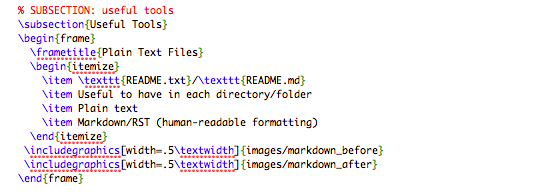
\includegraphics[width=.35\textwidth]{images/latex_before}
     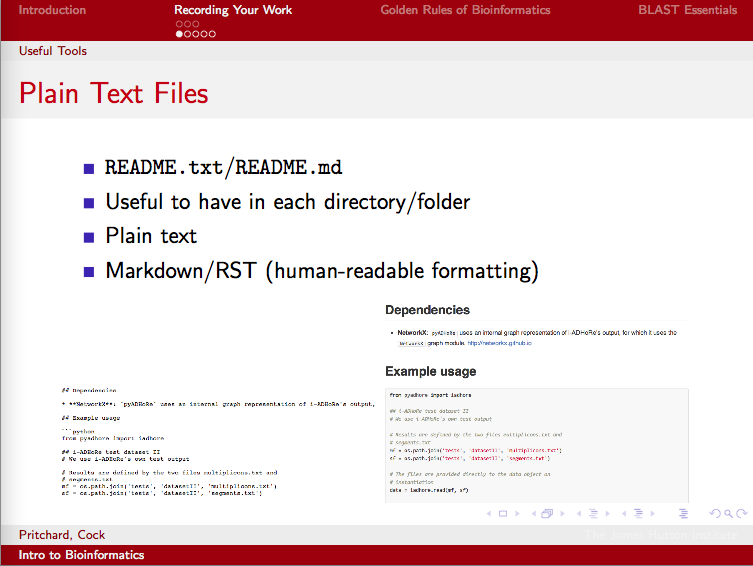
\includegraphics[width=.35\textwidth]{images/latex_after}     
  \end{center}
\end{frame}


%%%
% SECTION: Conclusions
\section{Conclusion}
  % Conclusions for the So You Want To Be a Bioinformatician slides

\subsection{Conclusion}
\begin{frame}
  \frametitle{In Conclusion}
  \begin{itemize}
    \item Bioinformatics is just biology using computers and mathematics
    \item You still need to ``do science" in the same way:
    \begin{itemize}
      \item Keep accurate records
      \item Plan and conduct experiments (with controls)
      \item Follow the literature
      \item Professional development
    \end{itemize}
  \end{itemize}
\end{frame}


% etc
\end{document}
